\section{BTB\_\-btac\_\-t::BTB\_\-btac\_\-t::BTB\_\-btac\_\-Entry\_\-t Struct Reference}
\label{structBTB__btac__t_1_1BTB__btac__Entry__t}\index{BTB\_\-btac\_\-t::BTB\_\-btac\_\-Entry\_\-t@{BTB\_\-btac\_\-t::BTB\_\-btac\_\-Entry\_\-t}}
Collaboration diagram for BTB\_\-btac\_\-t::BTB\_\-btac\_\-t::BTB\_\-btac\_\-Entry\_\-t:\nopagebreak
\begin{figure}[H]
\begin{center}
\leavevmode
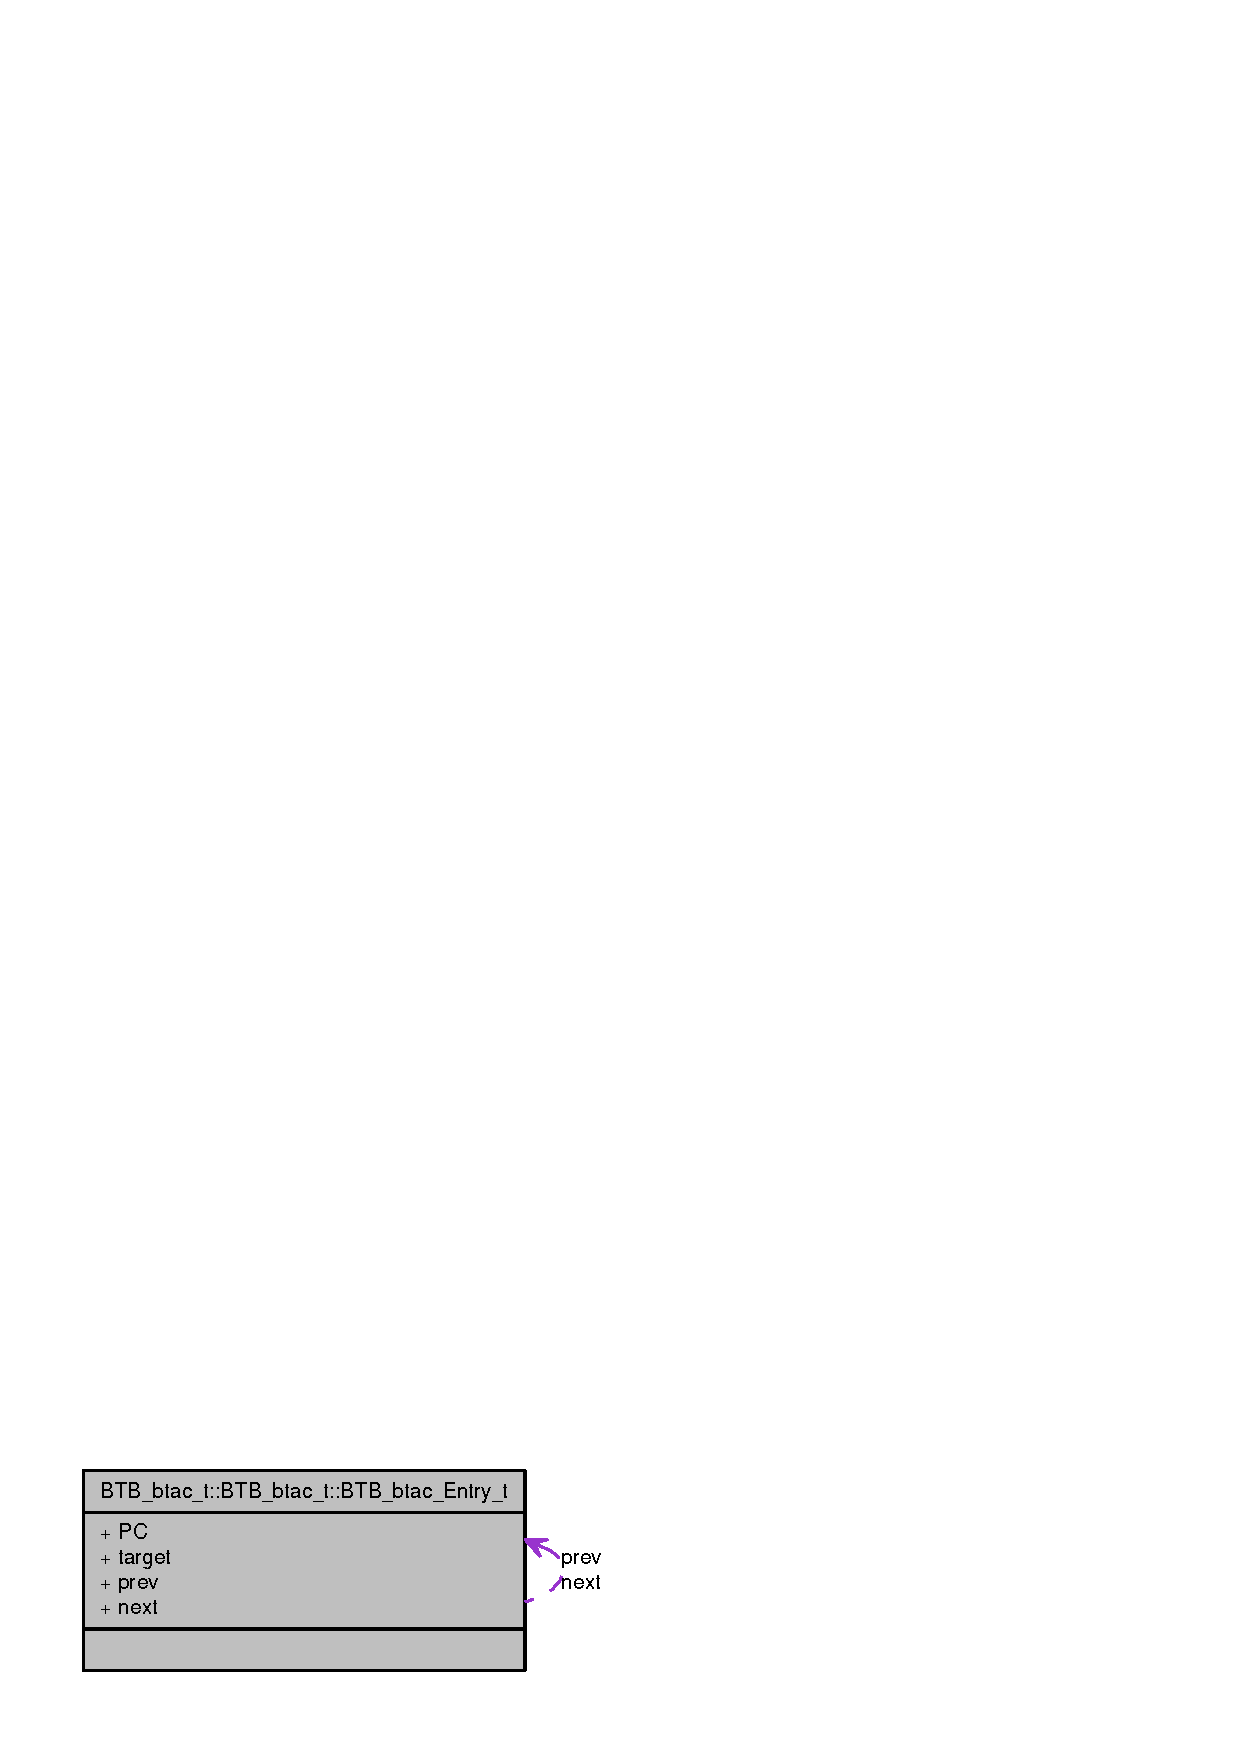
\includegraphics[width=293pt]{structBTB__btac__t_1_1BTB__btac__Entry__t__coll__graph}
\end{center}
\end{figure}
\subsection*{Public Attributes}
\begin{CompactItemize}
\item 
{\bf md\_\-addr\_\-t} {\bf PC}
\item 
{\bf md\_\-addr\_\-t} {\bf target}
\item 
struct {\bf BTB\_\-btac\_\-Entry\_\-t} $\ast$ {\bf prev}
\item 
struct {\bf BTB\_\-btac\_\-Entry\_\-t} $\ast$ {\bf next}
\end{CompactItemize}


\subsection{Detailed Description}


Definition at line 25 of file btb-btac.cpp.

\subsection{Member Data Documentation}
\index{BTB\_\-btac\_\-t::BTB\_\-btac\_\-Entry\_\-t@{BTB\_\-btac\_\-t::BTB\_\-btac\_\-Entry\_\-t}!next@{next}}
\index{next@{next}!BTB_btac_t::BTB_btac_Entry_t@{BTB\_\-btac\_\-t::BTB\_\-btac\_\-Entry\_\-t}}
\subsubsection[{next}]{\setlength{\rightskip}{0pt plus 5cm}struct {\bf BTB\_\-btac\_\-Entry\_\-t}$\ast$ BTB\_\-btac\_\-t::BTB\_\-btac\_\-t::BTB\_\-btac\_\-Entry\_\-t::next\hspace{0.3cm}{\tt  [read]}}\label{structBTB__btac__t_1_1BTB__btac__Entry__t_fa5dd7e22e2aca715904ff54dc36dad7}




Definition at line 30 of file btb-btac.cpp.

Referenced by BTB\_\-btac\_\-t::BTB\_\-btac\_\-t(), and BTB\_\-btac\_\-t::$\sim$BTB\_\-btac\_\-t().\index{BTB\_\-btac\_\-t::BTB\_\-btac\_\-Entry\_\-t@{BTB\_\-btac\_\-t::BTB\_\-btac\_\-Entry\_\-t}!PC@{PC}}
\index{PC@{PC}!BTB_btac_t::BTB_btac_Entry_t@{BTB\_\-btac\_\-t::BTB\_\-btac\_\-Entry\_\-t}}
\subsubsection[{PC}]{\setlength{\rightskip}{0pt plus 5cm}{\bf md\_\-addr\_\-t} BTB\_\-btac\_\-t::BTB\_\-btac\_\-t::BTB\_\-btac\_\-Entry\_\-t::PC}\label{structBTB__btac__t_1_1BTB__btac__Entry__t_d736a579cbea8059988ff8742e45e0b7}




Definition at line 27 of file btb-btac.cpp.\index{BTB\_\-btac\_\-t::BTB\_\-btac\_\-Entry\_\-t@{BTB\_\-btac\_\-t::BTB\_\-btac\_\-Entry\_\-t}!prev@{prev}}
\index{prev@{prev}!BTB_btac_t::BTB_btac_Entry_t@{BTB\_\-btac\_\-t::BTB\_\-btac\_\-Entry\_\-t}}
\subsubsection[{prev}]{\setlength{\rightskip}{0pt plus 5cm}struct {\bf BTB\_\-btac\_\-Entry\_\-t}$\ast$ BTB\_\-btac\_\-t::BTB\_\-btac\_\-t::BTB\_\-btac\_\-Entry\_\-t::prev\hspace{0.3cm}{\tt  [read]}}\label{structBTB__btac__t_1_1BTB__btac__Entry__t_bea75989d1f999e004bdf99b8f7eb46a}




Definition at line 29 of file btb-btac.cpp.

Referenced by BTB\_\-btac\_\-t::BTB\_\-btac\_\-t().\index{BTB\_\-btac\_\-t::BTB\_\-btac\_\-Entry\_\-t@{BTB\_\-btac\_\-t::BTB\_\-btac\_\-Entry\_\-t}!target@{target}}
\index{target@{target}!BTB_btac_t::BTB_btac_Entry_t@{BTB\_\-btac\_\-t::BTB\_\-btac\_\-Entry\_\-t}}
\subsubsection[{target}]{\setlength{\rightskip}{0pt plus 5cm}{\bf md\_\-addr\_\-t} BTB\_\-btac\_\-t::BTB\_\-btac\_\-t::BTB\_\-btac\_\-Entry\_\-t::target}\label{structBTB__btac__t_1_1BTB__btac__Entry__t_919a202963420ca65ca54e800db38b43}




Definition at line 28 of file btb-btac.cpp.

The documentation for this struct was generated from the following file:\begin{CompactItemize}
\item 
{\bf btb-btac.cpp}\end{CompactItemize}
